\documentclass[11pt, a4paper]{report}
\makeatletter
\def\input@path{{../../}}
\makeatother
\usepackage{../../styling}
\usepackage[backend=biber, style=numeric, sorting=none]{biblatex}
\DefineBibliographyStrings{english}{bibliography = {References}}
\usepackage{tocloft}
\usepackage{tabularx}
\usepackage{multicol}

% Reduce vertical space between the Contents title and first entry.
\setlength{\cftbeforetoctitleskip}{0pt}
\setlength{\cftaftertoctitleskip}{6pt}

\numberwithin{equation}{section}

% Uniform compact 2-column References block
\newcommand{\compactbib}{%
  \vspace{-16pt}%
  \enlargethispage{20pt}%
  \section*{References}%
  \vspace{-33pt}%
  \begingroup
    \begin{singlespace}%
      \begin{multicols}{2}%
        \scriptsize
        \setlength{\bibitemsep}{0pt}%
        \printbibliography[heading=none]%
      \end{multicols}%
    \end{singlespace}%
  \endgroup
}

\addbibresource{../../yuze_references.bib}

\title{Supply Chain Design}
\author{Yuze Jiang}
\date{\today}

\begin{document}

\pagenumbering{gobble}

\maketitle

\newpage

\pagenumbering{arabic}
\setcounter{page}{1}

\tableofcontents
\newpage

\chapterauthor{Supply Chain Design}{Yuze Jiang}

\section{Introduction}

This part of the report examines the supply chain design of a Formula Student "rabbit" vehicle used for autonomous emergency braking (AEB) testing.

The vehicle was originally developed for the acceleration event, where the objective is to achieve high acceleration over a short distance of approximately \SI{75}{\meter}. As a result, the design is optimised for short-duration, high-performance operation, with components such as the battery sized specifically for brief usage.

While such characteristics differ from those required in conventional racing applications, they align well with the requirements of AEB testing. In this context, the vehicle is used as a dynamic obstacle, repeatedly crossing the path of a test vehicle to evaluate detection and braking performance.

This shift in application fundamentally changes the nature of the system. Rather than focusing on one-off performance or large-scale production, the vehicle operates as part of a repeated testing cycle. Consequently, the primary challenge becomes maintaining continuous operation, where downtime directly limits testing capability.


Therefore, the supply chain must prioritise availability and rapid recovery, rather than minimising cost or inventory.

To structure the analysis, the report is divided into three levels: supply chain strategy, planning, and operation. These represent decisions over different time horizons, where strategy focuses on long-term structure over several years, planning considers medium-term decisions over months, and operation addresses short-term execution on a daily or weekly basis \cite{Supply_chain_lecture}.

\section{Supply Chain Strategy}

\subsection{Strategic Objective}

Strategy defines the long-term structure of the supply chain, within which planning and operational decisions are made. In this case, the strategy must be aligned with the uncertainty inherent in system operation.

Given the operational nature of the system, the supply chain is primarily evaluated based on its ability to maintain continuity rather than efficiency. This implies that the key objective is not to minimise cost or inventory, but to ensure that failures can be absorbed without interrupting the testing cycle. As a result, supply chain decisions are driven by recovery capability, including the availability of spare parts and response time. In this context, availability becomes the dominant design constraint, and trade-offs are made in favour of reducing downtime rather than optimising resource utilisation.

\subsection{System Framing}

Given that the primary objective is to maintain continuous operation, it becomes necessary to reconsider how the system is defined from a supply chain perspective.

The system can no longer be understood as a conventional production process. Instead of focusing on the manufacture and delivery of multiple units, it operates as a repeated testing cycle, where the same vehicle is used continuously over time. This fundamentally changes the nature of the supply chain. The key challenge is not how many units can be produced, but how reliably the system can continue to operate in the presence of failures. In this context, failures are expected as part of normal operation, and the system must support a cycle of testing, failure, and recovery rather than a linear production flow.

As a result, the supply chain is better understood as a process-oriented or service-oriented system, where value is generated through repeated operation rather than product delivery. This shifts the focus from output volume to system availability and continuity.

\subsection{Strategy Type}

Based on the operational characteristics of the system, the supply chain is best described as a combination of multiple approaches rather than a single conventional model.

\paragraph{Supply Chain Structure (Centralised vs Distributed)}

Structurally, the system is highly centralised, as all operations are concentrated around a single testing setup. From a market perspective, the overall service demand is relatively limited and geographically concentrated, which reduces the need for a distributed network. Introducing multiple testing locations would increase capital investment and operational complexity without providing significant benefits in responsiveness.

In practice, the use of a single testing site simplifies coordination and ensures consistency across repeated test cycles. Since the system is reused continuously rather than deployed across multiple locations, centralisation allows resources, equipment, and spare components to be concentrated in one place, improving both control and efficiency. This is particularly important for maintenance and recovery activities, which rely on immediate access to tools and spare parts. Overall, a centralised structure supports operational efficiency while avoiding unnecessary duplication of resources.

\paragraph{Sourcing Strategy (Outsourcing vs In-house)}

In terms of sourcing, the system adopts a partially outsourced approach. Most components are sourced externally, as the relatively low production volume does not justify the high capital investment required for in-house manufacturing. In contrast, selected activities are retained in-house where either customisation is required to meet specific performance needs or where processes are relatively low in complexity and capital requirement.

In practice, components that require specialised manufacturing capabilities, such as the motor and inverter, are sourced externally. Meanwhile, in-house activities focus on components requiring customisation, as well as processes that are critical for maintenance and recovery. For example, structural repair and assembly are carried out in-house, allowing immediate response to failures without relying on external suppliers, thereby reducing downtime. This approach balances cost efficiency with operational flexibility.

\paragraph{Operating Strategy (Lean vs Agile)}

From an operational perspective, the system aligns more closely with an agile supply chain. The operating environment is characterised by uncertainty, particularly due to failure events that occur unpredictably during testing. This makes responsiveness and flexibility more important than efficiency, as the system must be able to adapt to changing conditions and recover quickly from disruption.

In contrast to traditional lean systems, which rely on stable and predictable processes, this system cannot fully optimise for efficiency due to the variability introduced by failures. Instead, agility allows the system to respond effectively to unexpected events, particularly during recovery. However, elements of lean behaviour are still present in the preparation and execution stages, where processes are repetitive and structured. Overall, the system reflects a hybrid approach, where agile principles dominate under uncertainty while lean principles are applied where stability allows.

\paragraph{Flow Strategy (Push vs Pull)}

At the same time, the system exhibits a mixed push--pull behaviour. Certain components, particularly those with higher risk or longer disruption duration, require advance preparation and pre-positioned inventory, reflecting push-based planning. This ensures that critical failures can be addressed immediately without waiting for external supply.

In contrast, other components can be managed in a more reactive manner, where actions are triggered by failure events or operational demand. This pull-based behaviour reduces unnecessary inventory and allows resources to be used more efficiently. Importantly, the push--pull boundary is not fixed but varies across components depending on their risk profile. This flexible boundary allows the system to balance responsiveness and efficiency, ensuring that resources are allocated where they have the greatest impact on maintaining system continuity.

\paragraph{Conclusion}

Overall, the supply chain can be characterised as a centralised, agile, and failure-driven system, where decisions are adapted to the level of risk and uncertainty associated with different components. And the strategy reflects a strong alignment between system requirements and supply chain design, ensuring that operational continuity is maintained under uncertain conditions.

\section{Supply Chain Planning}

\subsection{Planning Framework}
\label{subsec:supply_chain_planning_framework}

Given the operational nature of the system, supply chain planning is driven by managing risk rather than forecasting demand or production volume.

The key consideration is how different failures affect the continuity of testing, particularly in terms of how likely they are to occur and how much downtime they introduce. As a result, planning decisions focus on prioritising resources towards components that have the greatest impact on system availability.  To structure this, the analysis considers three main factors: failure likelihood, impact on system operation, and recovery time. These together determine the level of preparation required for each component. This ensures that limited resources are allocated where they have the greatest effect on maintaining system continuity.

\subsection{Failure Mode and Effect Analysis (FEMA)}

To support the planning framework, a structured failure analysis is carried out using a simplified Failure Mode and Effects Analysis (FMEA)\cite{FMEA_lecture_notes}. Rather than focusing solely on downtime, this approach allows different failure modes to be linked to their likelihood, underlying causes, and operational impact.

For non-collision conditions, failure likelihood can be informed by component specifications and available engineering data, such as expected lifetime and operating limits. In contrast, collision-related failures are less predictable and cannot be directly obtained from standard data sources. Instead, they are assessed based on the physical characteristics of each component, including their exposure to impact, level of protection within the system, and their ability to withstand mechanical loads.

The FMEA is therefore used to compare components based on how frequently failures are expected to occur and how significantly they affect system continuity. As detailed quantitative data is not available, the analysis is applied in a qualitative and semi-quantitative manner, focusing on relative differences between components rather than precise numerical prediction.

A summary of the FMEA results for the powertrain components is presented in Table~\ref{tab:fmea}, illustrating how failure likelihood and recovery time combine to determine overall risk.

A detailed FMEA covering other subsystems is provided in the logbook.

\begin{table}[H]
\centering
\small
\renewcommand{\arraystretch}{1.5}

\caption{Failure Mode and Effect Analysis for Powertrain Component}
\label{tab:fmea}

\begin{tabularx}{\textwidth}{l X c X c}
\toprule
Component & Failure Mode (Non-collision) & Failure Prob (Non-collision) & Failure Mode (Collision) & Failure Prob (Collision) \\
\midrule
Electric Motor & Overheating Bearing wear & 0.001 & Impact-induced damage & 0.005 \\
Controller (VCU) & Overcurrent Firmware & 0.003 & Shock Connection fault & 0.008 \\
Inverter & Overheating IGBT failure & 0.002 & Impact-induced electrical fault & 0.01 \\
Drive Shaft & Wear Fatigue & 0.01 & Impact bending & 0.1 \\
Sprocket & Wear & 0.02 & Impact break & 0.2 \\
Chain & Fatigue Elongation & 0.02 & Impact failure & 0.2 \\
Differential & Gear Bearing wear & 0.002 & Impact-induced internal damage & 0.01 \\
Power Wiring & Loose Connector failure & 0.02 & Impact disconnection & 0.05 \\
\bottomrule
\end{tabularx}
\end{table}

\subsection{Risk Classification}

Building on the FMEA results, which provide a detailed view of individual component failures, a more aggregated perspective is required to support decision-making at the system level. While the FMEA highlights how each component behaves, it does not directly indicate how resources should be prioritised across the system.

To support decisions on whether and how spare parts should be prepared, a baseline scenario is first considered in which no spare parts are available, so that system recovery depends entirely on component replacement. Under this assumption, lead time is used as a proxy for recovery time, representing the full duration of disruption following a failure.

This approach effectively combines principles from failure analysis and supply chain planning. In particular, it reflects the general concept of risk as a function of likelihood and consequence, where failure probability represents the likelihood of disruption and lead time captures its impact in terms of system downtime.

\begin{figure}
    \centering
    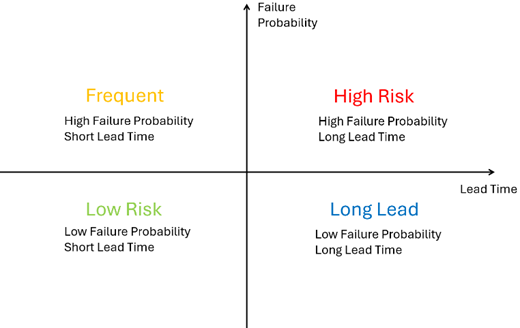
\includegraphics[width=0.5\linewidth]{figures/Conceptual_classification_of_component_risk.png}
    \caption{Conceptual classification of component risk}
    \label{fig:riskclassification}
\end{figure}

Based on this, components are classified according to two key factors: failure likelihood and lead time, which together determine how frequently disruptions occur and how long the system is affected when they do. A conceptual classification is first introduced in Figure~\ref{fig:riskclassification}, defining four categories based on these dimensions. The boundaries between categories are defined using median values, providing a consistent and relative basis for comparison.

The classification is applied to the system under both non-collision and collision conditions. Figure~\ref{fig:non-collision} presents the distribution under normal operation (non-collision conditions), while Figure~\ref{fig:collision} shows the corresponding distribution under collision conditions. This comparison highlights how certain components shift into higher-risk regions when exposed to impact.

\begin{figure}
    \centering
    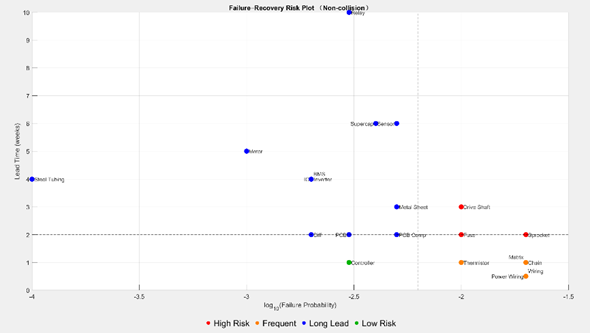
\includegraphics[width=0.5\linewidth]{figures/non_collision.png}
    \caption{Component classification under non-collision conditions}
    \label{fig:non-collision}
\end{figure}
%need update from Michael

From this representation, components can be grouped into four categories: high-risk components with both high failure likelihood and long lead time; frequent components that fail often but are relatively quick to recover; long lead-time components that fail less frequently but result in extended downtime; and low-risk components with both low failure likelihood and limited operational impact.

This classification provides a structured basis for prioritising components and directly informs subsequent decisions on spare part allocation.

\begin{figure}
    \centering
    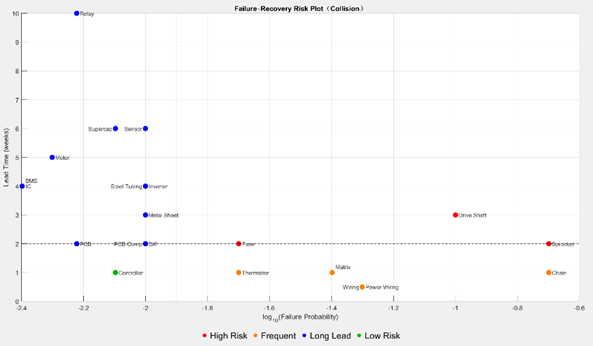
\includegraphics[width=0.5\linewidth]{figures/collision.png}
    \caption{Component classification under collision conditions}
    \label{fig:collision}
\end{figure}
%need update from Michael

\subsection{Spare Planning}

Based on the risk classification, spare part decisions are differentiated across components rather than applied uniformly. Since the objective is to maintain continuous operation, all components require some level of backup; however, the amount of inventory held depends on their impact on system continuity.

For high-risk components, which exhibit both high failure likelihood and long disruption duration, a push-based approach is adopted. Multiple spare units are maintained and pre-positioned to ensure that failures can be absorbed without interrupting the testing cycle. In this case, availability is prioritised over inventory cost.

For frequent components, which fail often but can be recovered quickly, a pull-based approach supported by a small buffer is more appropriate. Replacement is triggered by failure, while a limited number of spare parts is held to enable immediate recovery. This balances responsiveness with efficient use of inventory.

For long lead-time components, failures are less frequent but result in extended disruption when they occur. These components require advance preparation, typically in the form of at least one spare unit, to avoid excessive downtime.

For low-risk components, which have both low failure likelihood and limited impact on operation, a minimal inventory approach is sufficient. These components are largely managed on demand, with only a basic level of backup maintained to prevent unnecessary interruption.

Overall, the spare strategy is based on allocating inventory according to component risk, ensuring that stock is concentrated where it has the greatest effect on maintaining system continuity.

\subsection{Risk Mitigation}

While the spare strategy ensures availability through inventory, additional risk mitigation measures are applied to reduce system vulnerability without increasing stock levels. These measures focus on reducing either the likelihood of failure or the impact of disruption through design and sourcing decisions.

For components with significant supply risk, mitigation is primarily achieved by improving supply reliability. This includes the use of multiple suppliers or more standardised components, which reduces dependency on specific sources and limits exposure to supply disruptions.

For frequently failing components, mitigation focuses on reducing failure frequency and simplifying recovery. This can be achieved through improved component durability, standardisation, and ease of replacement, allowing the system to recover more quickly with minimal disruption.

In contrast, for low-risk components, additional mitigation is limited, as the cost and complexity of further intervention may not be justified by their relatively small impact on system performance.

Overall, these mitigation measures complement the spare strategy by reducing the system's reliance on inventory alone, enabling a more balanced and efficient allocation of resources.

\subsection{Conclusion}

The planning analysis shows that component prioritisation can be based on failure likelihood and disruption duration. By combining FMEA with risk classification, components are grouped according to their impact on system continuity. This provides a clear basis for allocating spare parts and defining preparation levels.

\section{Supply Chain Operation}

\subsection{Operational Flow}

\begin{figure}
    \centering
    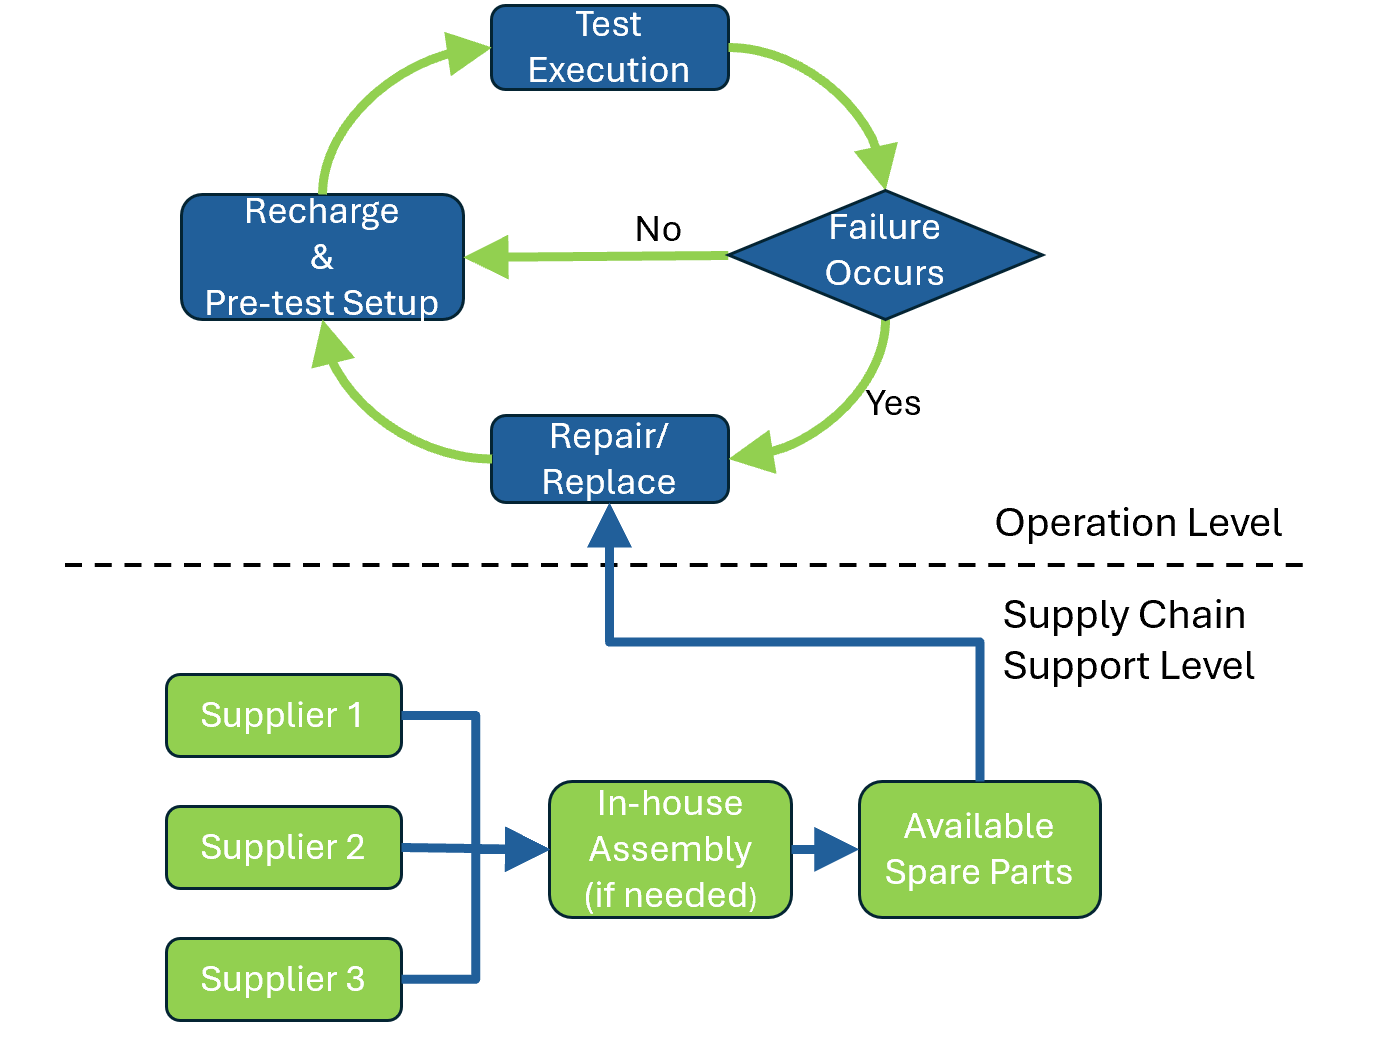
\includegraphics[width=0.5\linewidth]{figures/operation1.png}
    \caption{Operational cycle and supply chain support structure}
    \label{fig:operation}
\end{figure}

The operation of the system is illustrated in Figure~\ref{fig:operation}. The system operates as a closed loop, in which the vehicle is repeatedly used for testing rather than following a linear production process.

Each cycle consists of a preparation stage, including recharge and pre-test setup, followed by test execution. After each test, a decision point determines whether a failure has occurred. If no failure is detected, the system proceeds directly to the next cycle; otherwise, it transitions to repair or replacement before returning to operation.

This operational loop is supported by a supply chain layer, which ensures that spare parts are available when needed, enabling the system to recover and continue testing.

\subsection{Process Behaviour}

The operational cycle described in Figure~\ref{fig:operation} exhibits different characteristics across its stages and therefore cannot be represented by a single process model.

The preparation and test execution stages are highly structured and repeatable, with clearly defined procedures and consistent execution. These stages resemble lean operation, where efficiency and standardisation are prioritised due to the repetitive nature of the process.

In contrast, the recovery stage following a failure is inherently less predictable. The type and extent of damage can vary significantly, particularly under collision conditions, requiring flexible responses and case-by-case decision-making. This stage therefore exhibits characteristics of agile operation, where responsiveness and adaptability are prioritised over efficiency.

As a result, the system combines both lean and agile behaviours within the same operational cycle, with the dominant mode depending on the stage of operation.

\subsection{Downtime and Performance Constraints}

The performance of the system is primarily constrained by non-execution time, as any delay outside the test execution phase directly reduces testing throughput. A summary of the operational time distribution is presented in Table~\ref{tab:operation_time}.

\begin{table}[H]
\centering
\small
\renewcommand{\arraystretch}{1.5}

\caption{Summary of Operational Time Distribution}
\label{tab:operation_time}

\begin{tabularx}{\textwidth}{l X c c}
\toprule
Stage & Description & Time & Role in Process \\
\midrule
Recharge & Battery charging & $\sim$10 s & Non-value-added \\
Pre-test Setup & System checks and preparation & $\sim$430 s & Non-value-added \\
Test Execution & Dynamic crossing test & $\sim$36 s & Value-added \\
Recovery & Repair/replacement & 10 min--2 days & Non-value-added \\
\bottomrule
\end{tabularx}
\end{table}

From a customer value perspective, a value-added activity is defined as an activity that directly transforms the product or service in a way that the customer is willing to pay for. Activities that do not meet this criterion are classified as non-value-added, even if they are necessary for system operation.\cite{value_added}

Based on this definition, the test execution phase represents the primary value-added activity, as it directly contributes to the generation of meaningful testing data. In contrast, recharge, pre-test setup, and recovery constitute non-value-added time, as they do not directly create value from the perspective of the testing objective, despite being necessary for operation.

This classification follows the standard lean manufacturing distinction between value-added and non-value-added activities, where processes are analysed based on their contribution to customer value.

As shown in Table~\ref{tab:operation_time}, the pre-test setup stage accounts for a significantly larger portion of the cycle compared to the execution phase. This indicates that system throughput is not limited by the test itself, but by the activities required before and after each run. In addition, the recovery stage introduces substantial variability, ranging from short repairs to extended structural recovery, further increasing uncertainty in overall cycle time.

As a result, system performance is mainly influenced by the combined effect of preparation time and recovery variability, rather than by execution speed. Improving performance, therefore, depends on reducing non-value-added activities and managing disruption caused by failures.

\subsection{Process Improvements}

The analysis in the previous section shows that system downtime is primarily driven by the preparation and recovery stages. These two sources of delay require different approaches to improvement.

For the preparation stage, the process is highly structured and repeatable, making it suitable for lean-based improvements. Performance can be enhanced by reducing non-value-added activities through better organisation of the workspace, minimising unnecessary movement, and improving the layout and sequencing of tasks. These measures aim to streamline the preparation process and reduce the time required before each test cycle.

In contrast, the recovery stage can be viewed as a form of changeover process, where the system transitions from a failed state back to operation. This stage is less predictable and often requires component replacement or repair, making it a major contributor to downtime. In this context, principles similar to SMED (Single-Minute Exchange of Die) can be applied, where activities are divided into those that must be performed while the system is stopped (internal) and those that can be completed in advance (external). By shifting as many tasks as possible from internal to external, the effective downtime can be significantly reduced.

The use of a spare vehicle represents an extension of this approach. Instead of performing repair during downtime, a fully prepared backup system can be deployed immediately, allowing recovery to occur outside the operational cycle. This effectively converts part of the recovery process from an internal activity into an external one.
%talk about modular supply chain maybe(Paul)

It is important to note that this does not imply maintaining multiple complete backup systems. As established in the planning analysis, all components require at least a minimal level of spare availability. Rather than increasing the total amount of inventory, a single spare vehicle can be used to cover components that require immediate replacement, while additional spare parts are maintained selectively where needed.

Following replacement, the repaired vehicle can then be restored and reused as the spare system, allowing the spare resource to be rotated within the system. This approach enables rapid recovery while avoiding unnecessary duplication of resources.

\subsection{Key Activities}

While the previous section describes how the system operates, this section outlines the key activities required to support and manage the system in practice.

Due to the service-oriented nature of the system and the relatively low volume of operation, traditional procurement and supplier selection activities are less critical compared to conventional production systems. Instead, the focus shifts towards maintaining system availability and ensuring continuous operation through effective management of existing resources.

Inventory management is a central activity, involving the tracking and allocation of spare parts across different component categories. This ensures that critical components identified in the planning stage are available when required, while avoiding unnecessary duplication of inventory.

Maintenance and recovery activities are also essential, including post-test inspection, fault identification, and execution of repair or replacement procedures. Standardising these processes helps to reduce downtime and improve consistency in system recovery.

In addition, system monitoring plays an important role in supporting ongoing operation. Failure data can be recorded and analysed over time, allowing adjustments to spare allocation and risk prioritisation as more information becomes available.

Finally, while most components are sourced externally, sourcing-related activities focus on maintaining flexibility and reducing supply risk. This includes ensuring compatibility across different suppliers, monitoring supplier availability, and favouring standardised components where possible. These actions reduce dependency on specific sources and improve the system's ability to respond to supply disruptions. Overall, these activities enable the system to operate reliably in practice, ensuring that the supply chain effectively supports continuous testing.

\section{Conclusion}

The supply chain for the rabbit vehicle is driven by the need to maintain continuous operation under conditions of uncertainty, rather than to optimise production efficiency. By combining failure analysis with risk classification, components can be prioritised based on their impact on system continuity, providing a structured basis for decision-making.

This leads to a differentiated approach to resource allocation, where both inventory and mitigation efforts are focused on components that have the greatest effect on system downtime. In addition, operational improvements, such as the reorganisation of spare resources, further reduce disruption by enabling faster recovery.

Overall, the system can be characterised as a centralised, agile, and failure-driven supply chain, in which performance is determined by the ability to manage uncertainty and minimise interruption within a repeated operational cycle.

\section*{Appendix: Data Sources and Contributions}

The data used in the FMEA and subsequent analysis are derived from the engineering design of the project. These include component specifications, estimated failure behaviour, and recovery-related information.

The data for different subsystems were provided by team members responsible for their design:

\begin{itemize}
    \item Powertrain: Yuze Jiang
    \item Battery: Paul Vogelburg
    \item Wheels: Ziyang Xing
    \item Chassis: Toby McConnell
\end{itemize}

Detailed data sources should be provided in the references for each corresponding section.

\compactbib

\end{document}
